\documentclass[conference]{sty/IEEEtran}
\usepackage{times}
\usepackage{wrapfig}
\usepackage{tweaklist}
\usepackage{xspace}
\usepackage{graphicx}
\usepackage{subfigure}
\usepackage{tabularx}
\usepackage{amsmath}
\usepackage{amssymb}
\usepackage{url}


% numbers option provides compact numerical references in the text. 
\usepackage[numbers]{natbib}
\usepackage{multicol}
\usepackage[bookmarks=true]{hyperref}

\pdfinfo{
   /Author (Homer Simpson)
   /Title  (Robots: Our new overlords)
   /CreationDate (D:20101201120000)
   /Subject (Robots)
   /Keywords (Robots;Overlords)
}

\begin{document}

% paper title
\title{Classification of Objects of Daily Use Using Combined Color CHLAC and Global Radius-based Surface Descriptors}

% You will get a Paper-ID when submitting a pdf file to the conference system
\author{Author Names Omitted for Anonymous Review. Paper-ID [add your ID here]}

%\author{\authorblockN{Michael Shell}
%\authorblockA{School of Electrical and\\Computer Engineering\\
%Georgia Institute of Technology\\
%Atlanta, Georgia 30332--0250\\
%Email: mshell@ece.gatech.edu}
%\and
%\authorblockN{Homer Simpson}
%\authorblockA{Twentieth Century Fox\\
%Springfield, USA\\
%Email: homer@thesimpsons.com}
%\and
%\authorblockN{James Kirk\\ and Montgomery Scott}
%\authorblockA{Starfleet Academy\\
%San Francisco, California 96678-2391\\
%Telephone: (800) 555--1212\\
%Fax: (888) 555--1212}}


% avoiding spaces at the end of the author lines is not a problem with
% conference papers because we don't use \thanks or \IEEEmembership


% for over three affiliations, or if they all won't fit within the width
% of the page, use this alternative format:
% 
%\author{\authorblockN{Michael Shell\authorrefmark{1},
%Homer Simpson\authorrefmark{2},
%James Kirk\authorrefmark{3}, 
%Montgomery Scott\authorrefmark{3} and
%Eldon Tyrell\authorrefmark{4}}
%\authorblockA{\authorrefmark{1}School of Electrical and Computer Engineering\\
%Georgia Institute of Technology,
%Atlanta, Georgia 30332--0250\\ Email: mshell@ece.gatech.edu}
%\authorblockA{\authorrefmark{2}Twentieth Century Fox, Springfield, USA\\
%Email: homer@thesimpsons.com}
%\authorblockA{\authorrefmark{3}Starfleet Academy, San Francisco, California 96678-2391\\
%Telephone: (800) 555--1212, Fax: (888) 555--1212}
%\authorblockA{\authorrefmark{4}Tyrell Inc., 123 Replicant Street, Los Angeles, California 90210--4321}}


\maketitle

\begin{abstract}
The abstract goes here.
\end{abstract}

\IEEEpeerreviewmaketitle

\section{Introduction}

\section{Related Work}
\begin{itemize}
\item VFH
\item GRSD (Humanoids10GRSD)\cite{kalman1960new} 
\item Color CHLAC (Asako)
\end{itemize}

\section{System Overview}


\section{Feature Estimation}

\subsection{Color CHLAC}

\subsection{GRSD}
%
Compute radiuses as in \cite{Marton10CAD}.
Since these values have physical meaning, we can categorize surfaces using
simple, intuitive rules, into: planes (large $r_{min}$), cylinders (medium $r_{min}$,
large $r_{max}$), edges (small $r_{min}$ and $r_{max}$), rims (small $r_{min}$,
medium to large $r_{max}$), and spheres (similar $r_{min}$ and $r_{max}$).
Figure~\ref{fig:gfpfh} shows annotated the surface types.

Once all voxels are annotated locally using a geometric class, our
processing pipeline constructs a global feature by counting the transitions
between these local labels (and free space). Since we do not use raycasting
as previously in \cite{Humanoids} but consider only the direct neighbors
of each occupied cell, the computation of this \emph{simplified} GRSD is much faster.

\begin{figure}[htb!]
  \begin{center}
    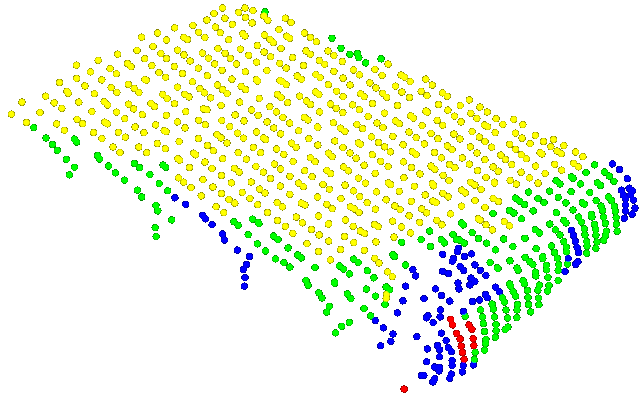
\includegraphics[width=.4\columnwidth]{figures/grsd/book.png}
\hfill
    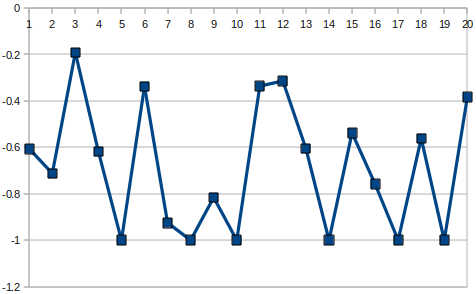
\includegraphics[width=.48\columnwidth]{figures/grsd/book_global.png} \\
\hfill
    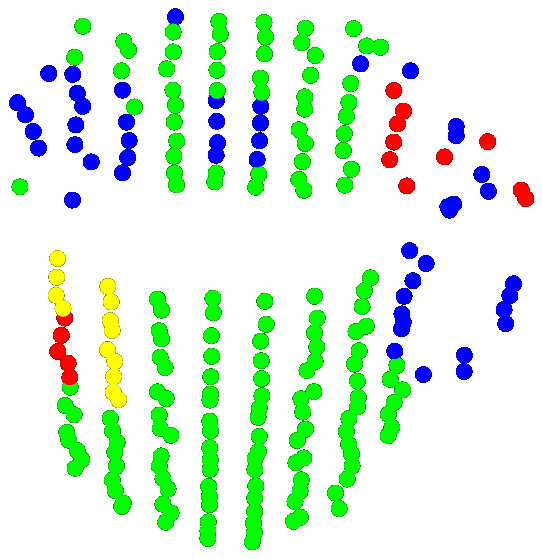
\includegraphics[width=.3\columnwidth]{figures/grsd/mug.png}
\hfill
    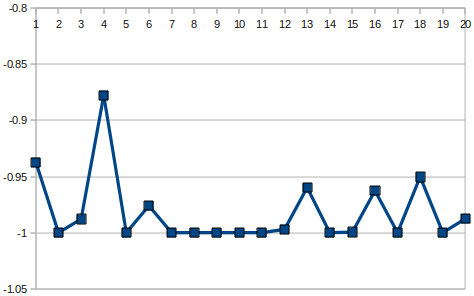
\includegraphics[width=.48\columnwidth]{figures/grsd/mug_global.png}
\caption{REDO: Example of RSD classes and GRSD plots for a big flat box (i.e. book, upper row) and a short cylinder (i.e. mug, bottom row).
The histogram bin values are scaled between -1 and 1 according to the
training data, and the colors represent the following local surfaces:
red - sharp edge (or noise), yellow - plane, green - cylinder, light blue -
sphere (not present), and dark blue - rim (i.e. boundary, transition between surfaces).
\emph{Best viewed in color.}
}
    \label{fig:gfpfh}
  \end{center}
\vspace{-2ex}
\end{figure}

\subsection{Comparison}
%
Same approach (if using rotation invariant Color-CHLAC), but different things are counted (color vs surface type). Also, GRSD considers free space as well.
\begin{figure}[htb!]
  \begin{center}
    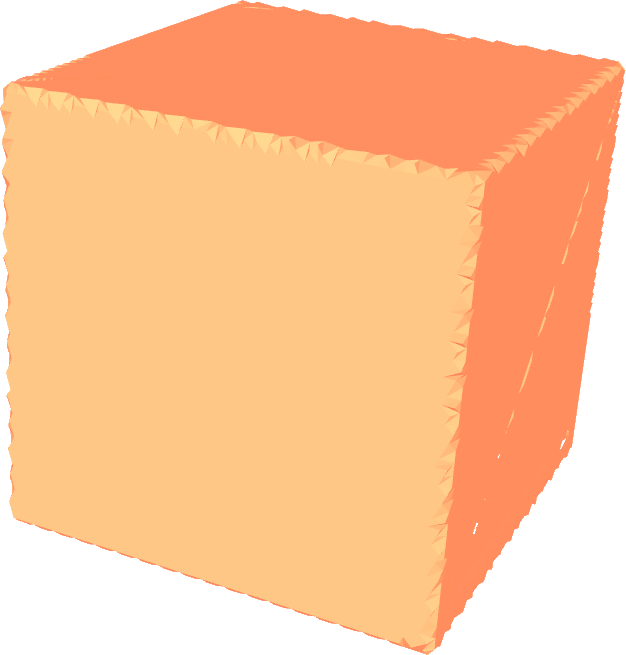
\includegraphics[width=.3\columnwidth]{figures/comparison/cube.png}
    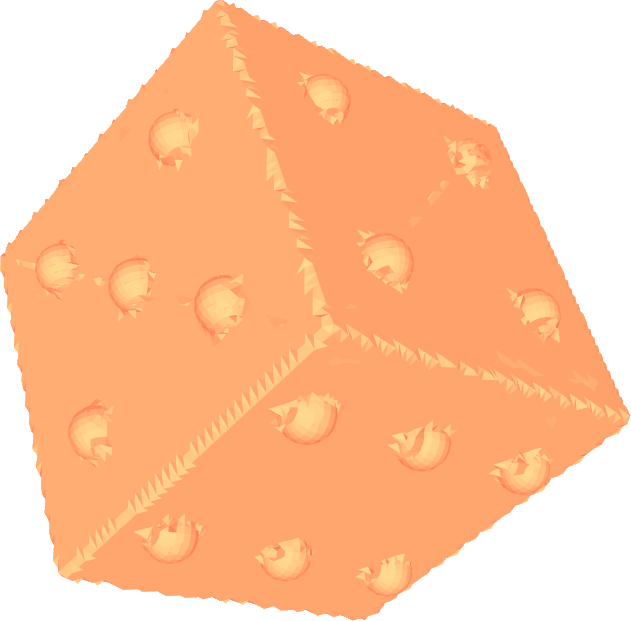
\includegraphics[width=.32\columnwidth]{figures/comparison/dice1.png}
    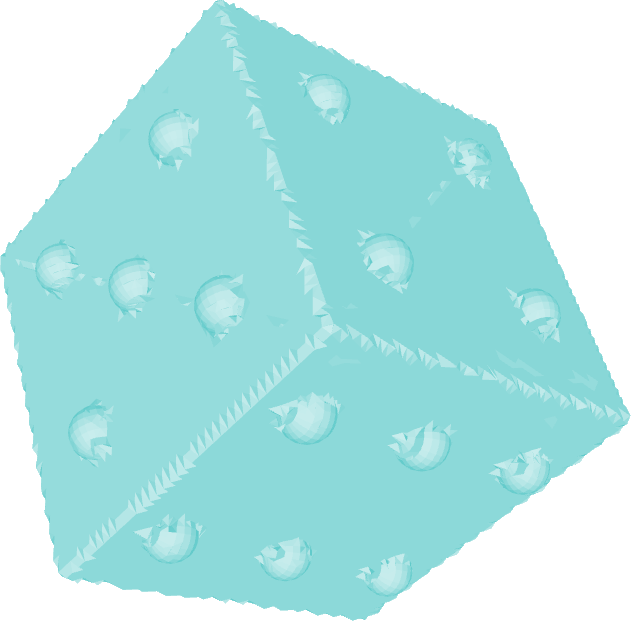
\includegraphics[width=.32\columnwidth]{figures/comparison/dice2.png}
    \caption{Color-CHLAC: can not differentiate the dice from the cube. GRSD: can not differentiate the different colors. Combination solves both.}
    \label{fig:comparison}
  \end{center}
\vspace{-2ex}
\end{figure}

\section{Classification Methods}

\subsection{Linear Subspace Method}
\subsection{Support Vector Machine-based Classification}


\section{Results}

\subsection{Data Acquisition and Training}
\begin{figure}[htb!]
  \begin{center}
    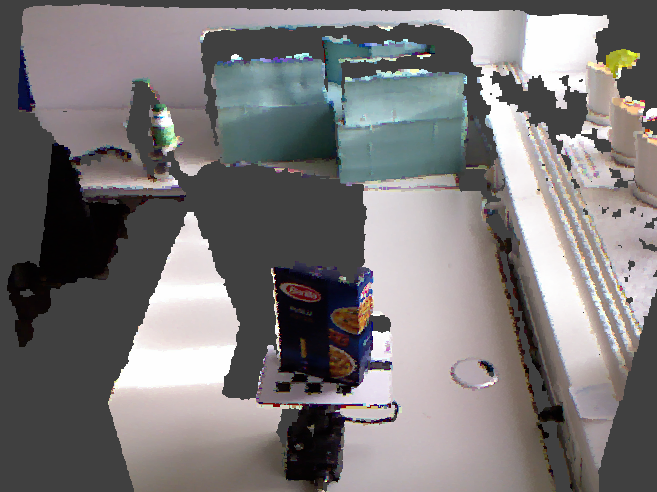
\includegraphics[width=.45\columnwidth]{figures/rot_table/barilla.png}
\hfill
    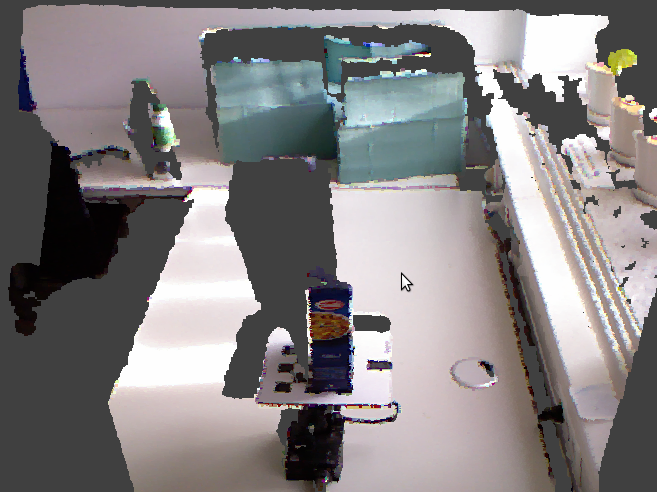
\includegraphics[width=.45\columnwidth]{figures/rot_table/barilla1.png} \\
\hfill
    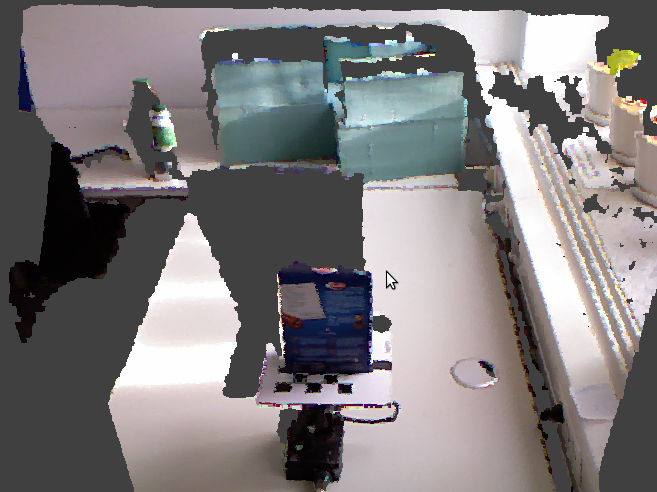
\includegraphics[width=.45\columnwidth]{figures/rot_table/barilla2.png}
\caption{Acquisition of Training Data}
    \label{fig:data_acquisition}
  \end{center}
\end{figure}
\subsection{Online Testing/Object Recognition}
\begin{figure}[htb!]
  \begin{center}
    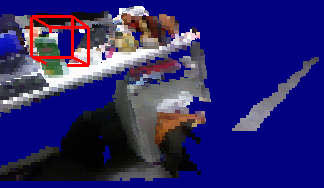
\includegraphics[width=.45\columnwidth]{figures/colorCHLAC/detection7.png}
\hfill
    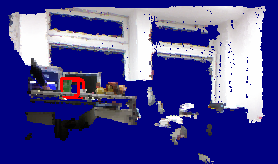
\includegraphics[width=.45\columnwidth]{figures/colorCHLAC/detection5.png} \\
\hfill
    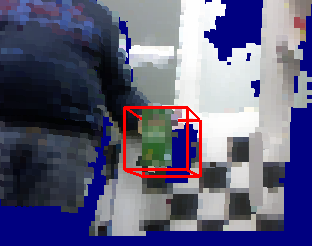
\includegraphics[width=.9\columnwidth]{figures/colorCHLAC/detection2.png}
\caption{An example of the detection of tetrahedral package of milk}
    \label{fig:milk_testing}
  \end{center}
\end{figure}


\section{Conclusions and Future Work} 
The conclusion goes here.

\section*{Acknowledgments}
CoTeSys
%% Use plainnat to work nicely with natbib. 

\bibliographystyle{plainnat}
\bibliography{references}

\end{document}


%TODO:
%Check the original template and see what the meant with the hyperlinks
